\section{Arbeitsjournal}
\label{sec:arbeitsjournal-ref}
Dieses Kapitel beinhaltet ein Review der Sprints und welche Tätigkeiten 
in diesen gemacht wurden.

\subsection*{Technologierecherche und Anforderungsliste}
\workday
    {1}
    {\ok Meilenstein 1 Erledigt. Alle Tasks abgeschlossen.}
    {
      Es wurde sich intensiv mit der Technologierecherche auseinandergesetzt.
      Dabei wurde versucht, wie im Design Thinking Prozess beschrieben, so breit wie möglich
      zu bleiben.
    }
    {
      Das Testat 1 konnte erfolgreich abgegeben werden mit verschiedenen Technologierecherchen in
      allen Bereichen.
    }
    \begin{figure}[H]
  \centering
  \begin{minipage}[t]{0.45\linewidth}
  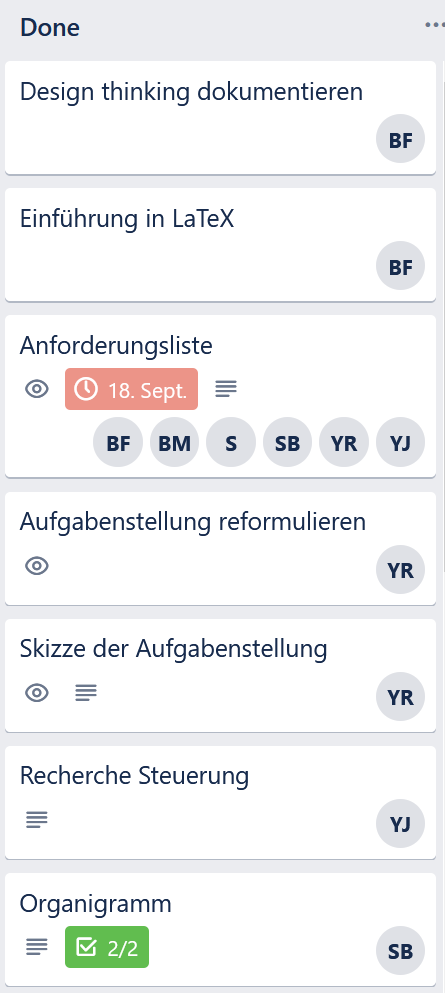
\includegraphics[width=0.7\textwidth]{img/Trello/Trello-Bord_1_Nr1.PNG}
  \caption{Scrum Board des Sprints 1, Teil 1}
  \label{Scrum Board 2.1}
  \end{minipage} 
  \hfill
  \begin{minipage}[t]{0.45\linewidth}
  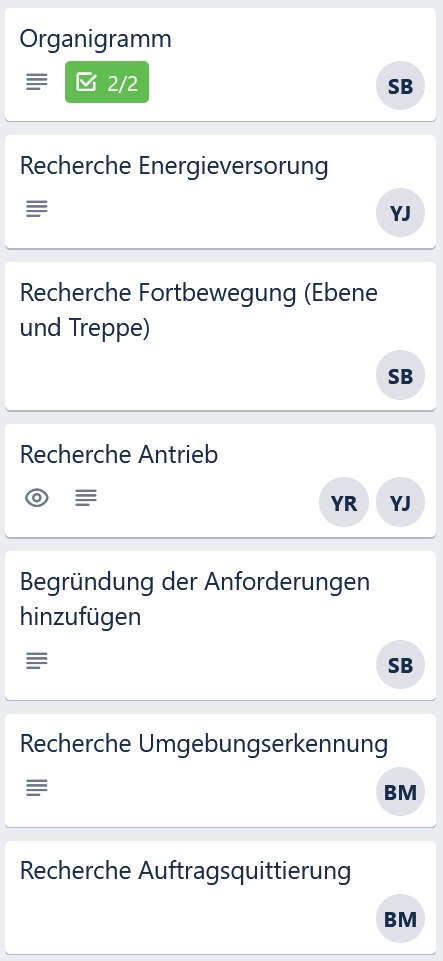
\includegraphics[width=0.7\textwidth]{img/Trello/Trello-Bord_1_Nr2.PNG}
  \caption{Scrum Board des Sprints 1, Teil 2}
  \label{Scrum Board 2.2}
  \end{minipage}
\end{figure}

\subsection*{Evaluation, Auswahl der optimalen Lösungskombination(en)}
\workday
    {2}
    {\ok Meilenstein 2 Erledigt. Bereits mit Meilenstein 3 angefangen.}
    {
      Im Meilenstein 2 wurden aus der Technologierecherche drei Lösungskonzepte erstellt
      und anschliessend evaluiert. Dabei wird der einfachste Ansatz weiterverfolgt. 
      Ganz nach dem Motto ``Keep it simple and stupid''.
    }
    {
      Aufgrund der zügigen Fortschritte bezüglich der ersten Evaluation, konnte rasch zur Evaluation der Teilkonzepte fortgeschritten werden.
    }

    
    \begin{figure}[H]
  \centering
  \begin{minipage}[t]{0.45\linewidth}
  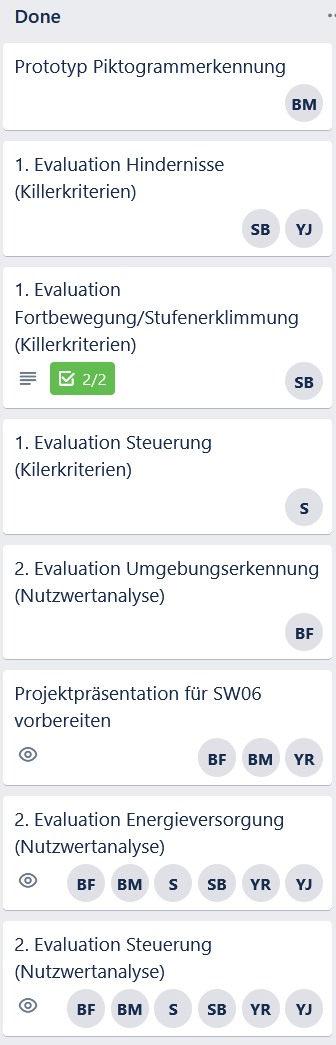
\includegraphics[width=0.7\textwidth]{img/Trello/Trello-Bord_2_Nr1.PNG}
  \caption{Scrum Board des Sprints 2, Teil 1}
  \label{Scrum Board 2.1}
  \end{minipage} 
  \hfill
  \begin{minipage}[t]{0.45\linewidth}
  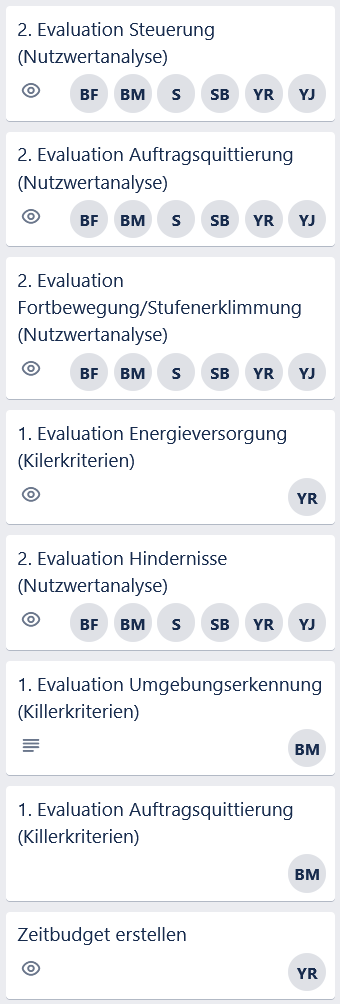
\includegraphics[width=0.7\textwidth]{img/Trello/Trello-Bord_2_Nr2.PNG}
  \caption{Scrum Board des Sprints 2, Teil 2}
  \label{Scrum Board 2.2}
  \end{minipage}
\end{figure}
    
    
\subsection*{Freigabe des Gesamtkonzeptes, Dokumentation zu 80\% erstellt}
\workday
    {3}
    {\ok Meilenstein 3 Erledigt.}
    {
      Die Dokumentation wurde soweit zu 80\% fertiggestellt. 
    }
    {
      Die Ideen konnten mithilfe der Funktionsmuster überprüft werden und geben einen verlässlichen Eindruck, wie der Roboter umgesetzt werden kann.
    }

    
    
        \begin{figure}[H]
  \centering
  \begin{minipage}[t]{0.45\linewidth}
  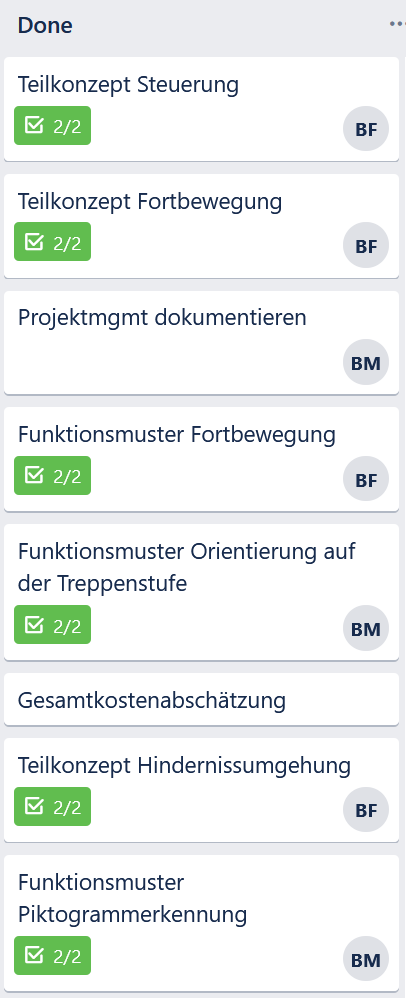
\includegraphics[width=0.7\textwidth]{img/Trello/Trello-Bord_3_Nr1.PNG}
  \caption{Scrum Board des Sprints 3, Teil 1}
  \label{Scrum Board 3.1}
  \end{minipage} 
  \hfill
  \begin{minipage}[t]{0.45\linewidth}
  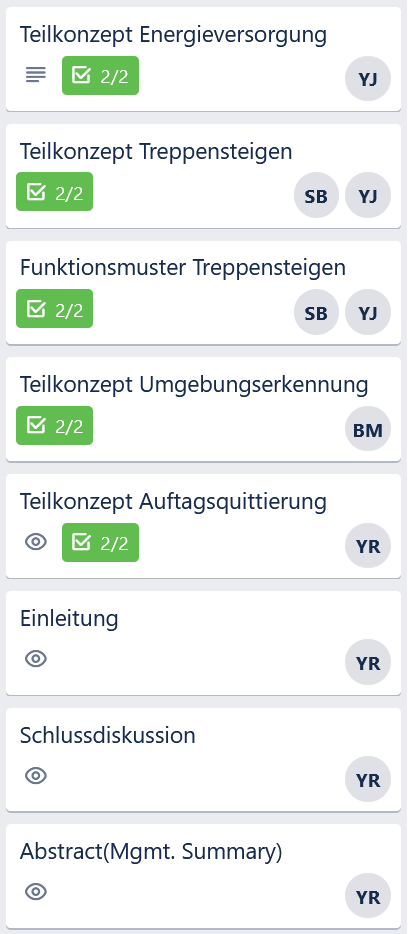
\includegraphics[width=0.7\textwidth]{img/Trello/Trello-Bord_3_Nr2.PNG}
  \caption{Scrum Board des Sprints 3, Teil 2}
  \label{Scrum Board 3.2}
  \end{minipage}
\end{figure}